\label{sec:evolutionarystaghunt}
Evolutionary games constist a population of agents that are randomly matched 
over time to play a stage game. So, in an evolutionary interpretation of the 
stag hunt game, the stage game is the SH game. 
Usually, the number of agents is assumed to be large such that on the hand, 
the effect of a single individual on the population is small, and on the
other hand, the interaction happens anonymously.
Populations can either be \textit{monomorphic} or \textit{polymorphic}.
Monomorphic populations consist of agents that are only able to play pure
strategies, whereas in polymorphic populations mixed strategies are allowed.
In the following, the focus will be on monomorphic populations as they have
a straightforward interpretation and the main implications do not differ. 
Formally, let $p_j(t) \geq 0$ denote the number of individuals in 
the population playing strategy $j \in \{1,2\}$ at time $t \in \realnumb$ and 
let $P = p(t) = p_1(t) + p_2(t)$ describe the total number of all individuals 
in the population. Note, $P =p(t)\ \forall t$ meaning that the population 
is not growing. The vector $\vec{x}(t) = \left(x_1(t),x_2(t)\right)
=\left(\frac{p_1(t)}{p(t)},\frac{p_2(t)}{p(t)}\right)$ is called the state 
vector of the population at time $t \in \realnumb$. 
Each component of the population state vector represent the share of agents 
choosing a specific strategy. As the individuals can only choose between 
strategy one and two in our example, it holds that  $x_2(t) = 1-x_1(t)$. 
Mentioned earlier, this enables a new interpretation of mixed strategies,
because $\vec{x}(t)$ is an element of the mixed strategy space $\Delta$.
Hence, mixed strategies in monomorphic games are simply the state
of the population, which in the SH game is the division of players on the two
pure strategies. This has, however, little relevance for the interpretation
in the traditional game \parencite[914-915]{rubinstein_comments_1991}.

Out of convenience, let the expected payoff 
to a strategy $i \in \{1,2\}$ of an individual randomly matched
against another individual in the current population state at time $t$, 
$\vec{x}(t)$, be denoted by $\hat{F}^i(\vec{x}) = \hat{F}(e_i,\vec{x})$. 

The next section will motivate \textit{revision protocols}, a rule to
which agents are ``programmed'' or ``wired'' \parencite{gintis_game_2000}, 
opposed to any rationality assumption. 
\subsection{Revision Protocols}
\label{sec:revisionprotocols}
This section motivates the use of revision protocols to
model the behavior of agents.
In contrast to the traditional approach, agents in evolutionary game theory, 
are usually not able to calculate best-replies, 
nor are they observing the information relevant
to perform that calculations.
Revision protocols formalize the idea that agents are following a certain
rule by which they change there strategy. 
The following derivation is due to \textcite{sandholm_population_2010}. 
Typically it is assumed that agents have an inner alarm clock 
which rings at a rate R following an exponential distribution. 
Of course, this does not translate 
to economic applications in individuals having literal clocks around their
wrist, but illustrates the idea of a randomly occuring chance to reconsider
their strategy choice.
The agents' clocks are assumed to be independent of each other such that
individuals chance to revise does not dependent on others.
Whenever the clock of an agent rings, he
receives a revision opportunity which means that he changes his strategy
with the probability $\frac{\rho_{ij}}{R}$, where
$\rho_{ij}(F_i(\vec{x}),\vec{x})$ is called the conditional switch rate,
representing the rule by which agents change from strategy 
$i$ to strategy $j$. 
In a two-strategy game there are two conditional switch rates, $\rho_{12}$ 
describing rate of switching from strategy 1 to 2 and $\rho_{21}$, 
rate for switching from strategy 2 to 1. For $\rho_{ii}$ no actual switch 
happens.
Switch rates result in first, different individual behavior rules, but 
secondly also in different dynamics for the whole population. An evolutionary
dynamic describes the change of the population vector $x(t)$ in time. 
The derivation of the dynamic can be done for a general conditional switch 
rate.
Every agent receives $R dt$ revision opportunities, i.e. the clock rings, 
in a time interval $[0,dt]$ as it follows a Poisson distribution with
mean $Rdt$ \parencite[123]{sandholm_population_2010}. 
If the population in the stag hunt game is at state $\vec{x}$, the number 
of agents currently playing strategy $i$ receiving a revision opportunity 
during the time interval of length $dt$ is $Px_i R dt$. As 
\textcite{sandholm_population_2010} argues, this is an approximation because
the state of the population $\vec{x}$ may change during the time interval $dt$.
With the probability for an agent playing strategy $i$ switching to strategy
$j$, one gets for the expected number of switches for strategy $i$ during 
$[0,dt]$ across the population,  $P x_i \rho_{ij} dt$. 
In a two strategy game, the change in the number of agents in the population 
playing strategy 1 is determined by agents switching to strategy 2 
and agents with strategy 2 switching to 1. Hence, one gets:
\begin{align} 
        Pdx_1 =  \underbrace{-Px_1 \rho_{12}dt}_{\text{Switches from 1 to 2}} 
        + \underbrace{Px_2 \rho_{21}dt.}_{\text{Switches from 2 to 1}}
\end{align}
Dividing by $P$ and $dt$ leaves us with the differential equation for
the change in the share of agents playing strategy 1, 
$\dot{x_1} =\frac{dx_1}{dt}$. 
The sum of the time derivatives of population shares must equal zero and so
$\dot{x}_2(t) =- \dot{x}_1(t)$.
There are different plausible revision protocols studied in the literature. 
\textcite[128,129,178]{sandholm_population_2010} discusses various forms of 
this revision protocols, such as logit choice, comparison to average payoff 
and best response 
protocol, all with different properties concerning informational 
burden and the
properties the dynamics have. With an eye to the implied dynamic, the 
\textit{pairwise proportional imitation} protocol will be outlined . 
It assumes, that whenever an
agent receives a revision opportunity he randomly gets to know 
another agent's strategy and its payoff received in the current 
state of the population. 
The switching probability of an agent is proportional to the 
excess payoff the other agent had over his strategy. 
Formally, 
\begin{align}
        \label{eq:pairwiseproportionalimitation}
        p_{ij}(F_i(\vec{x}),\vec{x}) =
                \begin{cases}
                        x_j(F_j(x) -F_i(x)) &\ , \text{for } F_j(x) - F_i(x) > 0 \\
                        0 &\ , \text{else}.
                \end{cases}
\end{align}
As a metaphor illustrating this revision protocol, I want to tell the 
story of traders on a marketplace.
Suppose the traders interact on a market selling some 
good, implicitly playing a game with each other. The strategies may be the
way they organize their market stall or what position on the market they 
choose. Each trader usually does not
observe the strategies other traders use to sell things, because the market
place is large and the bustle going on complicated. 
So a trader is usually committed to a strategy he got to know a while ago.
However, occasionally as he returns to his tavern, he sometimes gets to meet 
another trader. Being proud of their earnings, they boast about their 
individual strategy. In this way, they get to know
other traders strategies and as they all dream of a live in pageantry,
they might imitate the other traders. 
However, they are more likely to imitate traders with a higher payoff 
compared to theirs, as such traders feel superior and thus, are the 
loudest in the tavern. 

Plugging the conditional switch rate of the pairwise imitation protocol 
\eqref{eq:pairwiseproportionalimitation} into the equation for the change 
of the population share playing strategy 1, $\dot{x}_1(t)$, leads to the 
\textit{replicator dynamics}:
\begin{alignat}{2}
        \label{eq:replicatorrev} 
        \dot{x}_1 &= 2 x_1 x_2 (F_1(x) - F_2(x)) \\
                  &= 2 x_1 ((1-x_1) F_1(x) - x_2 F_2(x)) \\
                  &= 2 x_1 (F_1(x) - \bar{F}(x)) 
\end{alignat}
This equation fully describes the evolution of the population in time.
Properties and the connection to the stage game are discussed in the next
section.

\subsection{Replicator Dynamics}
\label{sec:replicatordynamic}
The Replicator Dynamic, one of most popular dynamics in 
evolutionary game theory, has a wide range of applications and 
attractive properties, such as population genetics and ecology, abiogenesis and
of course game theory \parencite[203]{hofbauer_evolutionary_1998}. 
It was mathematically formulated by \textcite{taylor_evolutionary_1978}, 
the biological concept replicator was introduced in 1982 by Dawkins 
\parencite{dawkins_extended_2016}.
As discussed above, the replicator dynamic can be motivated by different 
revision protocols. Using matrix notation, one finds 
for the strategies $j \in \{1,2\}$
\begin{alignat}{2}
        \dot{x}_j &= x_j\left(\left(x^T A\right)_j -
                \left(x^T A x\right)\right). 
        \label{eq:replicator}
\end{alignat}
The lack of the factor $2$, comparing it with equation 
\eqref{eq:replicatorrev}, is due to the derivation. In fact, any
positive transformation of the payoff matrix and hence the payoff function
results only in a change in speed in the replicator dynamic
\parencite[73]{weibull_evolutionary_1997}.
The growth of the share $\dot{x}_j(t)$ at time $t \in \realnumb$ depends 
on the current share in the population of strategy $j$ and the 
excess payoff of that strategy, the difference between the expected 
payoff to strategy $j$ against the current state of the population and the
average payoff across the whole population.
Intuitively, the share of a strategy in the population increases (decreases) 
if the strategy yields a higher (lower) than average payoff. 
This property of a (deterministic) evolutionary dynamic is called 
\textit{Positive correlation} \parencite{sandholm_population_2010}. 
\todo{pagenumber}
Another property of the replicator dynamic is the low data requirement. As 
seen in the previous section, it is not necessary to assume that an agent
gets to know the payoffs of all agents in the population.
It was sufficient to assume that he gets to know the payoff of one random 
player. 
Contrary to the interpretation that agents with such revision protocols 
are "boundedly rational", \textcite{gintis_game_2000}  argues 
that ``this is very misleading, because the real issue is the 
distribution of the information'' \parencite[273]{gintis_game_2000}. 
The argument goes, that even if they were not ``bounded'' they 
could not calculate since they do not have more information. 
One drawback of the replicator dynamic for certain applications, especially
for biologists, is the lack of mutation, a random error in the replication 
process.\todo{cite hofbauersigmund}
 Indeed, the deterministic replicator dynamic does not incorporate 
any such effect. A strategy that has not existed or has vanished from the 
population will not be in a future state of the population. 
That means, that if in a population state only a 
subset $S' \subset S$ of the 
set of pure strategies is used, any future population state can also only 
contain strategies from this subset $S'$. Hence, if a strategy in 
the stag hunt game vanishes, the population state is in one of the two pure 
Nash equilbria. It is practical for further use to express the replicator 
dynamics for the parametrized SH game using the matrix in equation 
\eqref{eq:matrix} and define $x_1(t) := x,\ x_2(t) = 1-x$:
\begin{alignat}{2}
        \label{eq:replicatorpara}
        \dot{x} := \varphi(x) &= x^2(a-b+2d-2c) - x^3(a-b+d-c) -x(d-c) \\
                              &= x^2(\alpha_1+2\alpha_2) 
        - x^3(\alpha_1+\alpha_2) - x(\alpha_2)
\end{alignat}
The last step follows by using local shifts to the matrix $A$ from section
\ref{sec:traditionalconcepts}. This does not change the dynamic at all 
\parencite[73]{weibull_evolutionary_1997}. The polynominal $\varphi(x)$ is
of degree $3$ and contains all information about the dynamic. Actually, 
outlined in the following, it tells which state the population converges to.
For the parameter set $a=5, b=3, c=0, d=2$ the graph of $\varphi(x)$ is 
plotted in figure \ref{fig:polynominal}. 
\todo{Description of the graph, roots e.t.c.}
\ref{fig:polynominal}.
\begin{figure}[h]
        \centering
        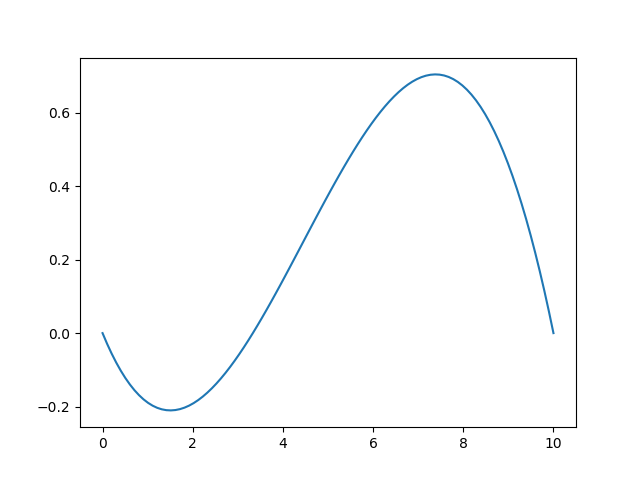
\includegraphics[scale=0.5]{polynominal.pdf}
        \caption[Polynominal of the Replicator Dynamic]{$\varphi(x)$ for the parameter setting $a=5, b=3, c=0, d=2$}
        \label{fig:polynominal}
\end{figure}
For the purpose of analyzing the properties of the replicator dynamic, it is 
useful to introduce some vocabulary used in dynamical system theory. 

A solution through an initial state $x_0$ of the dynamical system is called a 
\textit{trajectory}, whereby it is distinguished between a forward trajectory 
for $t \rightarrow \infty$ and backward trajectory for $t \leftarrow \infty$.
Analytical solutions, i.e. a solution one can express with the use of
basic functions, can only be derived for simple cases. 
It is easier to solve the differential equation numerically using some
computer software. 
However, the existence and uniqueness of a solution through
any initial state for the replicator dynamic is guaranteed by the theorem 
of \textit{Picard-Lindel\"of}, theorem 6.1 in 
\textcite[74]{weibull_evolutionary_1997}. 

The natural question that arises once a solution is obtained, is whether there 
is a connection between the evolutionary dynamic and the equilibria in the 
stage game. To see this, consider the concept of a fixed point.
A point $x^* \in \realnumb^2$ of a dynamic system, such as the replicator 
dynamic in \eqref{eq:replicator}, is called a fixed point
if $\dot{x}(t) = \varphi(x^*) = 0$ i.e. it stays in the current state for all 
$t \rightarrow + \infty $. 
Analyzing \eqref{eq:replicatorpara}, this happens if either a strategy
is not present in the population or the excess payoff of a strategy is zero. 
In the stag hunt game, the fixed points of the
dynamic coincide with the Nash equilibria of the stage game, 
$\varphi(x^*) = 0$ for $x^* \in \{0,\frac{\alpha_2}{\alpha_1+\alpha_2},1\}$. 
It suffices to calculate the roots of the polynominal $\varphi(x)$, either
numerical or, as the Nash equilibria are usually calculated beforehand,
reducing the degree by polynominal division. In general, the replicator 
dynamic lacks the \textit{Nash stationarity} property and hence there are 
games with fixed points which are not Nash\footnote{For a trivial example, 
consider the prisoners dilemma in \ref{fig:pd}. A population only consisting of 
cooperating agents stays in that state, which is not a Nash equilibrium even 
though it is Pareto-dominating.} \parencite{sandholm_population_2010}.
Concerning fixed points, one is usually interested if the fixed points of 
a dynamic system are stable in terms of some disturbance of the system. 
There are different approaches to stability. A quite strict and useful one 
in the stag hunt game is \textit{asymptotic stability}. 
It essentially requires that a system in a specific fixed point returns 
to the fixed point after a perturbation happened.
Hence, the system tends to move back to an asymptotically stable fixed point
once disturbed. Formally, a $\epsilon$-perturbation of 
\eqref{eq:replicatorpara} is a trajectory of the system with the initial
condition $x_0$ at some ball $B_\epsilon(x)$ of radius $\epsilon >0$ and 
$x_0 \neq x^*$. The fixed point $x^*$ is then called \textit{asymptotically
stable} if there exists an $\epsilon$-perturbation for that $x(t) \rightarrow
x^*$ as $t \rightarrow \infty$. 
The \textit{basin of attraction} of a fixed point $x^*$ is defined as the set 
of points $x_0 \in \realnumb$ for which a trajectory through $x_0$ approaches 
the fixed points $x^*$. In the one dimensional case, this is simply the range 
of $x$ for that any solution to the differential equation with the initial 
conditions in this range converges to the fixed point. With the following 
theorem independently contributed by \cite{hartman_lemma_1960} and 
\cite{grobman_homeomorphism_1959}, one can easily 
find the asymptotically stable fixed points in the stag hunt game:
\begin{mydef}
        If a one-dimensional dynamical system $\dot{x}(t) = \varphi{x}$ 
        has a hyperbolic fixed point $x^*$, $x^*$ is asymptotically stable
        if its linearization 
        $\dot{x}(t) = \frac{\partial\varphi(x)}{\partial x} := \varphi'(x)$ 
        is asymptotically stable. 
        A fixed point is called hyperbolic in one-dimension if 
        $\varphi'(x^*) \neq 0$ and the linearization is stable at that
        point if $\varphi'(x^*) < 0$.
\end{mydef}
The solution to the linearization can be analytical derived by 
a standard tool for differential equation - seperation of variables and 
integration.
The linearization around the fixed point $x^*$ is accordingly
$x(t)= x(0) e^{\varphi'(x^*)t}$, where $x(0)$ denotes the 
initial condition, i.e. the share of agents choosing strategy 1 in the 
beginning.
Applying the theorem to \eqref{eq:replicatorpara}, one finds that the 
fixed point $x=0$ corresponding to the Nash equilibrium of hunting hare, is 
asymptotically stable, since $\varphi'(0) = - \alpha_2 <0$. 
The linearization around the fixed point is $x(t) = x(0) e^{-\alpha_2 t}$, 
which clearly approaches zero as $t \rightarrow \infty$. 
Similarly, the Nash equilibrium 
of hunting stag at $x=1$ is a asymptotically stable fixed point as
$\varphi'(1) = -\alpha_1 <0$ with linearization $x(t) = x(0) e^{-\alpha_1 t}$.
However, the linearization theorem cannot be used for the mixed Nash 
equilibrium, hence the dynamical system is not hyperbolic there, 
$\varphi'(\frac{\alpha_2}{\alpha_1+\alpha_2}) = 0$. Nevertheless, suppose 
there is some $\epsilon$-perturbation of the system  \todo{Voooodoooo}
 with $x_0= \frac{\alpha_2}{\alpha_1+\alpha_2}+ \epsilon$ and 
 $\frac{\alpha_1}{\alpha_1+\alpha_2} > \epsilon > 0$. Plugging this into
 \eqref{eq:replicatorpara} one sees that $\dot{x} >0$, the population share
 grows monotonically for every $\epsilon$, converging to the fixed point 
 $x = 1$. Conversely, for $0 > \epsilon > \frac{\alpha_2}{\alpha_1+\alpha_2}$,
 $\dot{x} < 0$ and so the population share of agents 
 playing strategy 1 decreases monototically, until it reaches the 
 fixed point $x=0$. This is also shown in figure \ref{fig:basinofattraction}.
 \todo{Better description of the graphic}
 The horizonal line marks the mixed-strategy fixed point at $75\%$ for the
 parameter setting $\alpha_1 = 1$ and $\alpha_2=3$. If the population starts
 at this fixed point it by definiton stays there without any disturbance. 
 But any invasion of individuals with a uniform strategy leads away from
 this fixed point, resulting in convergence to one of pure strategy equilibria.
 The use of the word invasion is not by coincidence. It clearly shows the 
 connection of the evolutionary stable strategy of the stage game to the 
 stable fixed points of the dynamic. In fact, one can prove that this is not
 only true in the simple stag hunt, but it holds also under general settings.
 \todo{Folk theorem of evolutionary game theory}
\begin{figure}
        \centering
        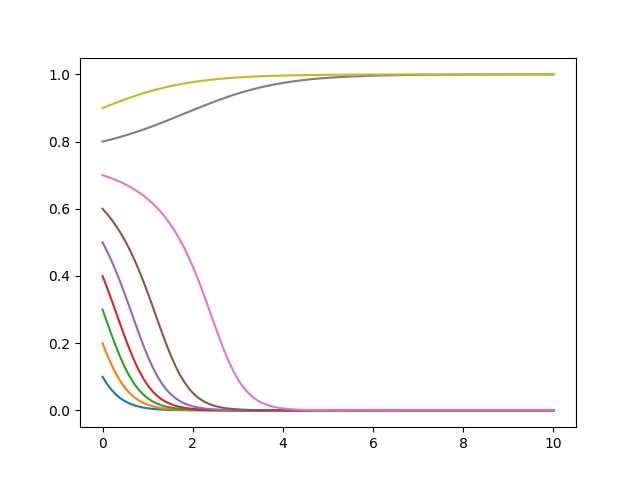
\includegraphics[scale=0.5]{basinofattraction.pdf}
        \caption[Replicator dynamic of the stag hunt game]{Replicator dynamics in the stag hunt game for 
                $\alpha_1=1,\ \alpha_2=3$ with different initial conditions}
                \label{fig:basinofattraction}
\end{figure}

Concering the equilibrium selection, the evolutionary approach with replicator
dynamic has a definite answer. The population will reach one of the three
Nash equilibria depending on the initial condition. 
However, an equilibrium not asymptotically stable is rather implausible,
because it only emerges from one initial condition, where the population
is already exactly in that population state. 
Intuitively, one additional agent playing
a pure strategy suffices to get the population state moving to one of the
pure equilibria. As the model outlined here is only a deterministic
approximation, any stochastic shock would lead to such a disturbance and hence
would start convergence to one of the states with evolutionary stable 
strategies.
The population converges to the stag hunting or the hare
hunting equilibrium if the initial conditions lie in their basin of attraction.
As discussed, the population converges to the state $x=1$, the stag hunting 
equilibrium of the stage game, for all initial conditions 
$x_0 \in (\frac{\alpha_2}{\alpha_1+\alpha_2},1]$. Any trajectory of the 
dynamical system with initial conditions 
$x_0 \in [0,\frac{\alpha_2}{\alpha_1+\alpha_2})$ lead to the hare hunting
equilibrium. Interestingly, one observes another connection of the 
dynamic with the stage game. The basin of attraction is larger for the
risk-dominating equilibrium. By definition \eqref{eq:riskdom}, 
the hare hunting equilibrium risk-dominates if $\alpha_2 > \alpha_1$,
so in fact the basin of attraction is larger. With the parameter setting shown
in figure \ref{fig:basinofattraction},$75\%$ of the possible initial 
conditions lead to the risk-dominant equilibrium, whereas only $25\%$ of the 
initial conditions lead to the payoff-dominant equilibrium. 
The equilibrium selection is determined by the position of the initial
condition. However, it is not clear what specifies the initial conditions. 
If for example the agents choose a random strategy in a first round of the 
game, independently of each other, one can say that the equilibrium with the
larger basin of attraction, the risk-dominant equilibrium, is more likely 
reached. \todo{what does evolutionary game theory tell about initial condition} 
Giving an exact answer which equilibrium will be selected through the dynamic
process, this approach still leaves us with the problem of what agents 
choose in a first round one-shot game. Section \ref{sec:experimentalevidence} 
summarizes evidence found in laboratory stag hunt game concerning the 
one-shot game strategy choice and so the justification for initial conditions.
